\chapter{Pendolo di Kater e caduta libera}
\section{Introduzione}
L'obiettivo dell'esperimento è misurare l'accelerazione gravitazionale $g$ attraverso due dei possibili metodi e confrontarli. 

\section{Pendolo di Kater}
\subsubsection{Introduzione}
\begin{wrapfigure}{R}{0.28\textwidth}
  \begin{center}
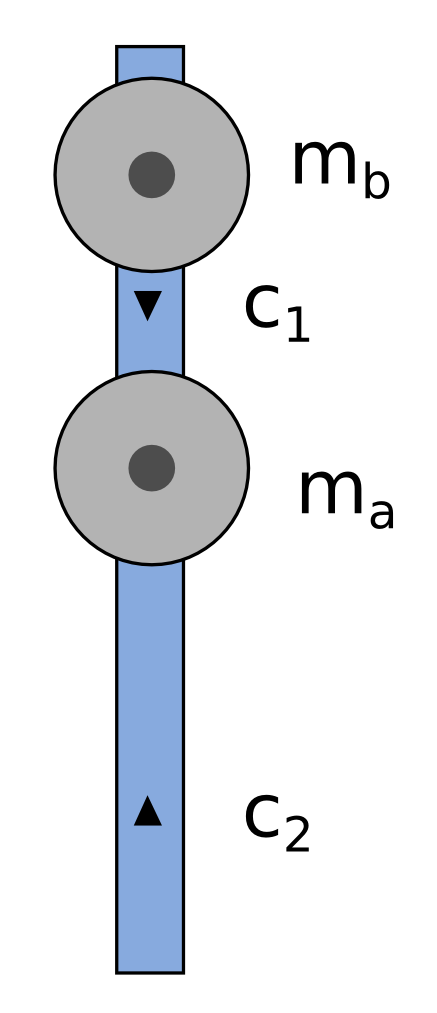
\includegraphics[scale=0.7]{../grafici/kater/kater.png}
  \end{center}
  \caption*{Il pendolo di Kater}
\end{wrapfigure}

Il pendolo di Kater è un pendolo fisico che può essere messo in oscillazione su due punti $c_1,\ c_2$ non coincidenti con il suo baricentro $G$. Il pendolo è costituito da un'asta rigida, due masse $m_a = 1400g$, $m_b=1000g$, e due coltelli, posizionati nei punti $c_1$ e $c_2$. La massa $m_a$ è mobile, e la sua distanza viene fatta variare rispetto a $c_1$. Dopodiché vengono misurati e riportati in tabella i periodi di oscillazione del pendolo, facendolo oscillare prima su $c_1$ e poi su $c_2$.

Il periodo del pendolo dipende ovviamente dalla posizione del baricentro rispetto al punto di sospensione. Chiamando $h_i$ la distanza del punto $i\in\{1,2\}$ dal baricentro:

$$ T_i = 2 \pi \sqrt{\frac{L_i}{g}} = 2 \pi \sqrt{\frac{I_i}{m gh_i}}$$

dove $L_i$ è la lunghezza ridotta del pendolo, $m$ è la massa totale e $I_i$ il momento d'inerzia del pendolo appeso per il punto $i$-esimo.
\\
Se si individuano i due punti nel quale il periodo $T_1 = T_2$ allora l'equazione si riduce a:

$$ T_0 = \ 2 \pi \sqrt{\frac{D}{g}}$$

La distanza $D= h_1 + h_2 $  è nota con grande precisione, e nel nostro caso è $D=99.4\ cm$. Misurando quindi il periodo $T_0=T_1=T_2$, possiamo calcolare $g$.
$$ g = \frac{4\pi^2D}{T^2}$$
\subsection{Procedimento}

In questo esperimento abbiamo utilizzato i seguenti strumenti:
\begin{itemize}
  \item Un metro a nastro, con sensibilità $1\ mm$
  \item Un cronometro digitale con fotocellula, che ha una precisione di $\pm 0.1 \cdot 10^{-3}\ s$
\end{itemize}

A questo punto abbiamo posto in oscillazione il pendolo dal coltello $c_1$ e misurato $T_1$; abbiamo poi ripetuto l'operazione per il coltello $c_2$, misurando $T_2$, e ripetuto la misura 10 volte al fine di stimare i migliori valori con i corrispondenti errori associati, mediante metodi statistici (media e deviazione standard).

Mantenendo fissa la massa $m_b$ ad una distanza $d = 15.4\ cm$ sopra il coltello in $c_1$ (all'estremità dell'asta), allontaniamo o avviciniamo la massa $m_a$, e ripetiamo le misure.

La massa $m_a$ viene spostata per cercare una posizione in cui $T_1 \simeq T_2$, ovvero quando si è in una condizione per la quale $L\simeq h_1+h_2$. 

\subsection{Dati}
Nella tabella sono raccolti tutti i periodi $T_1,T_2$ misurati in secondi. $d$ è la distanza tra il coltello $c_1$ e la massa $m_a$. \footnote{In tabella sono state riportate tutte le cifre significative che venivano lette nella fotocellula}
\begin{center}
\begin{tabular}{*{8}{c}}
$d$& $6.9\ cm$ & $11.7\ cm$ & $13.5\ cm$  & $15.0\ cm$ & $17.9\ cm$ & $85.0\ cm$ & $81.9\ cm$ \\
\midrule
 \textbf{Coltello 1}&& & & & & \\
&2.1197 &2.0040&2.0279 &1.9809 & 1.9211 & 1.9934 & 1.9735\\
 &2.1125&2.0041 &2.0029&1.9796 & 1.9207 & 1.9932 & 1.9744 \\
 &2.1179&2.0043 &2.0021&1.9816 & 1.9264 & 1.9931 & 1.9746 \\
 &2.1204&2.0062 &2.0042&1.9794 & 1.9253 & 1.9932 & 1.9755 \\
 &2.1189&2.0060 &2.0026&1.9821 & 1.9113 & 1.9932 & 1.9765 \\
 &2.1129&2.0052&2.0012&1.9805 & 1.9278 & 1.9934 & 1.9769 \\
&2.1125 &2.0050&2.0014&1.9802 & 1.9278 & 1.9937 & 1.9770 \\
&2.1131 &2.0061&2.0008&1.9804 & 1.9277 & 1.9941 & 1.9760 \\
 &2.1143&2.0046&2.0036&1.9810 & 1.9278 & 1.9937 & 1.9754 \\
 &2.1131&2.0058&2.0005& 1.9831 & 1.9278 & 1.9935 & 1.9750 \\
 \midrule
$\bar{x}$& 2.1158 & 2.0085 & 2.0021 & 1.9806 & 1.9244 & 1.9935 & 1.9755\\
$\sigma$ & 0.0032 & 0.0019 & 0.0012 & 0.0102 & 0.0053 & 0.0003 & 0.0011\\
\midrule
\textbf{Coltello 2} && & & & & \\
&2.0279&2.0041&1.9983 &1.9934 & 1.9882 & 1.9946 &	1.9802 \\
&2.0284&2.0043&1.9983 &1.9946 & 1.9902 & 1.9939 &	1.9812 \\
&2.0289&2.0062&1.9967 &1.9911 & 1.9907 & 1.9943 &	1.9820 \\
&2.0289&2.0060&1.9978 &1.9919 & 1.9908 & 1.9941 &	1.9818 \\
&2.0288&2.0052&1.9978 &1.9940 & 1.9907 & 1.9940 &	1.9819 \\
&2.0288&2.0050&1.9986 &1.9923 & 1.9907 & 1.9952 &	1.9813 \\
&2.0288&2.0061&1.9986 &1.9939 & 1.9888 & 1.9954 &	1.9816 \\
&2.0288&2.0046&1.9988 &1.9934 & 1.9898 & 1.9943 & 1.9818 \\
&2.0286&2.0058&2.0001 &1.9914 & 1.9898 & 1.9947 & 1.9812  \\
&2.0286&2.0040&1.9994 &1.9958 & 1.9878 & 1.9941 & 1.9810 \\
 \midrule
$\bar{x}$& 2.0827 & 2.0053 & 1.9984 & 1.9932 & 1.9832 & 1.9945 & 1.9814\\
$\sigma$ & 0.0003 & 0.0009 & 0.0009 & 0.0015 & 0.0017 & 0.0005 & 0.0005\\
\bottomrule
\end{tabular}
\end{center}

\subsection{Analisi}
I periodi $T_1$ e $T_2$ sono ovviamente funzione di $d$, essendo funzione dei momenti d'inerzia e della posizione del baricentro. I valori che ci interessano sono quelli in cui $T_1(d) = T_2(d)$.

L'equazione ha tre soluzioni, ma per semplicità, abbiamo deciso di concentrarci sulla prima, avendo cura di non considerare il caso banale $h_1=h_2$. Di seguito il grafico il quadrato del periodo in funzione di $d$ ($T_2$ in verde, $T_1$ in nero).

\begin{center}
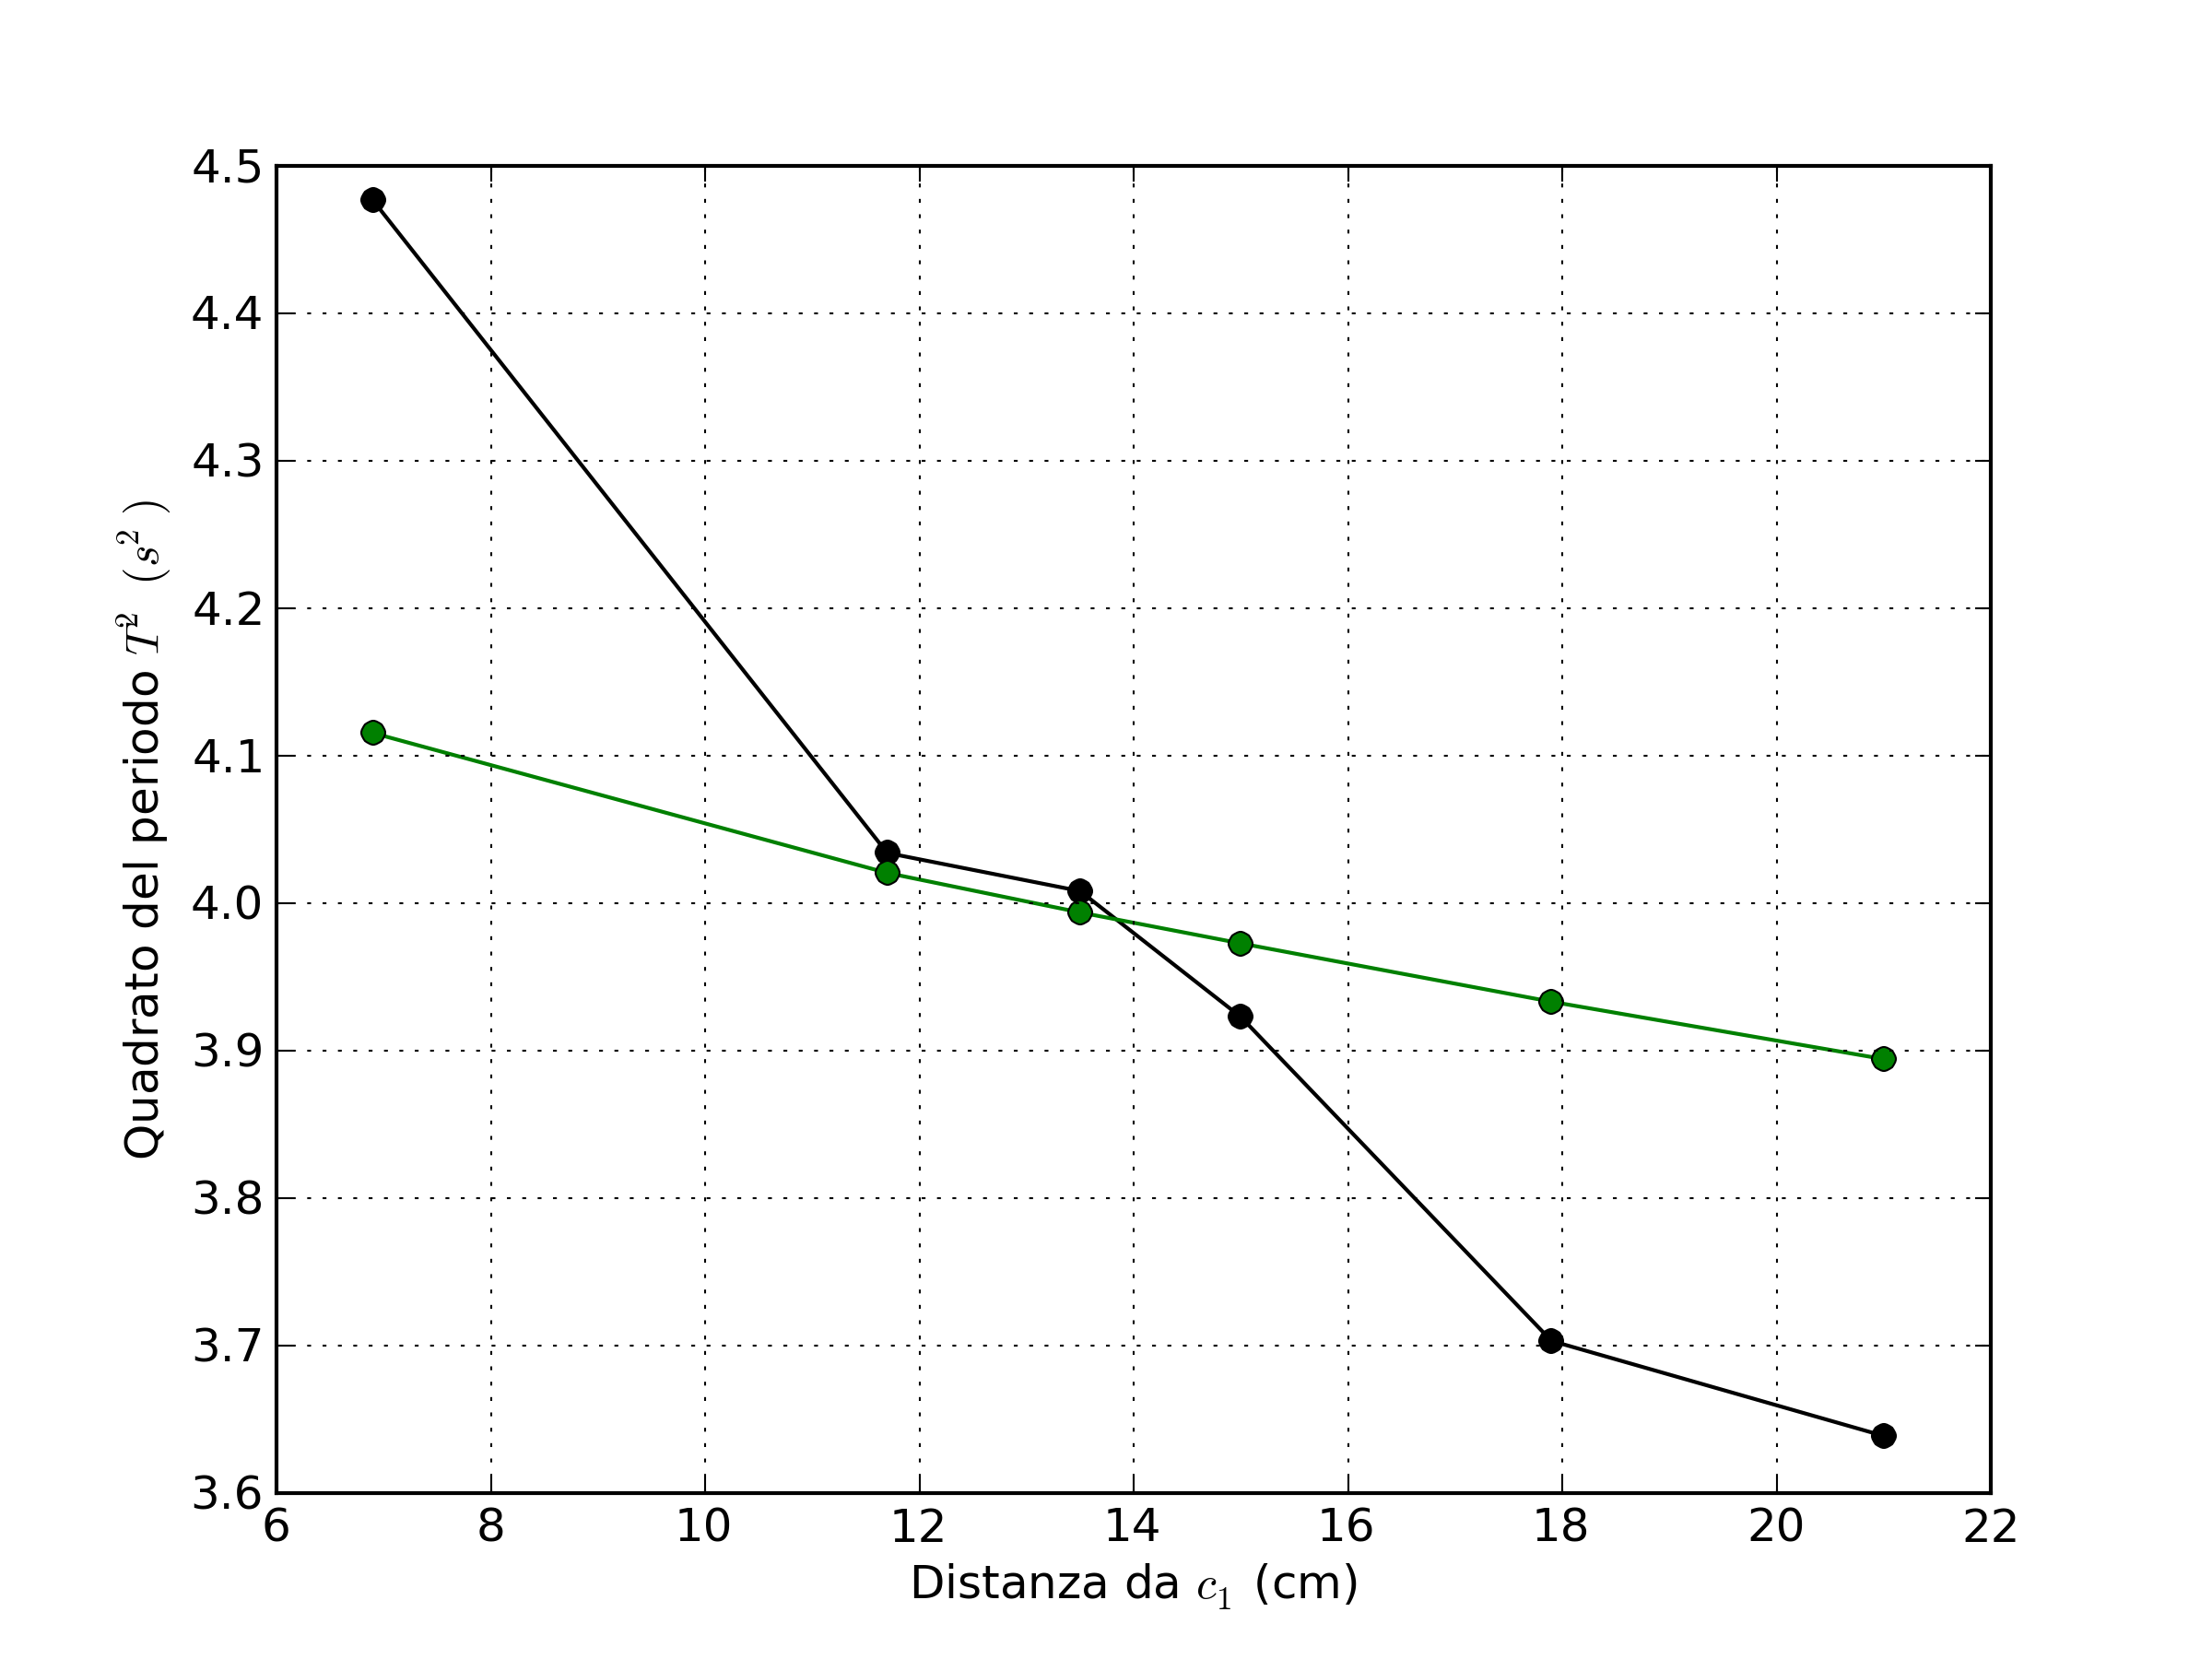
\includegraphics[scale=0.60]{../grafici/kater/kater-punti-raw.png}
\end{center}

La spezzata ha il solo scopo di collegare i punti al fine di rendere più leggibili i dati sperimentali.\\

Per ricercare il miglior punto di intersezione minimizzando l'errore, abbiamo deciso di considerare le misurazioni dei periodi delle cinque distanze più vicine al valore che sembrava maggiormente plausibile (in questo caso abbiamo scelto 13.5 cm) e abbiamo calcolato, per ognuna di queste, le differenze tra i periodi $T_1$ e $T_2$.

Scegliendo poi di considerare la posizione $d$ in funzione delle differenze di periodo, possiamo interpolare questi dati con una retta, e l'intercetta così trovata sarà ovviamente il valore cercato di $d$ tale che $T_1 = T_2$.

\begin{center}
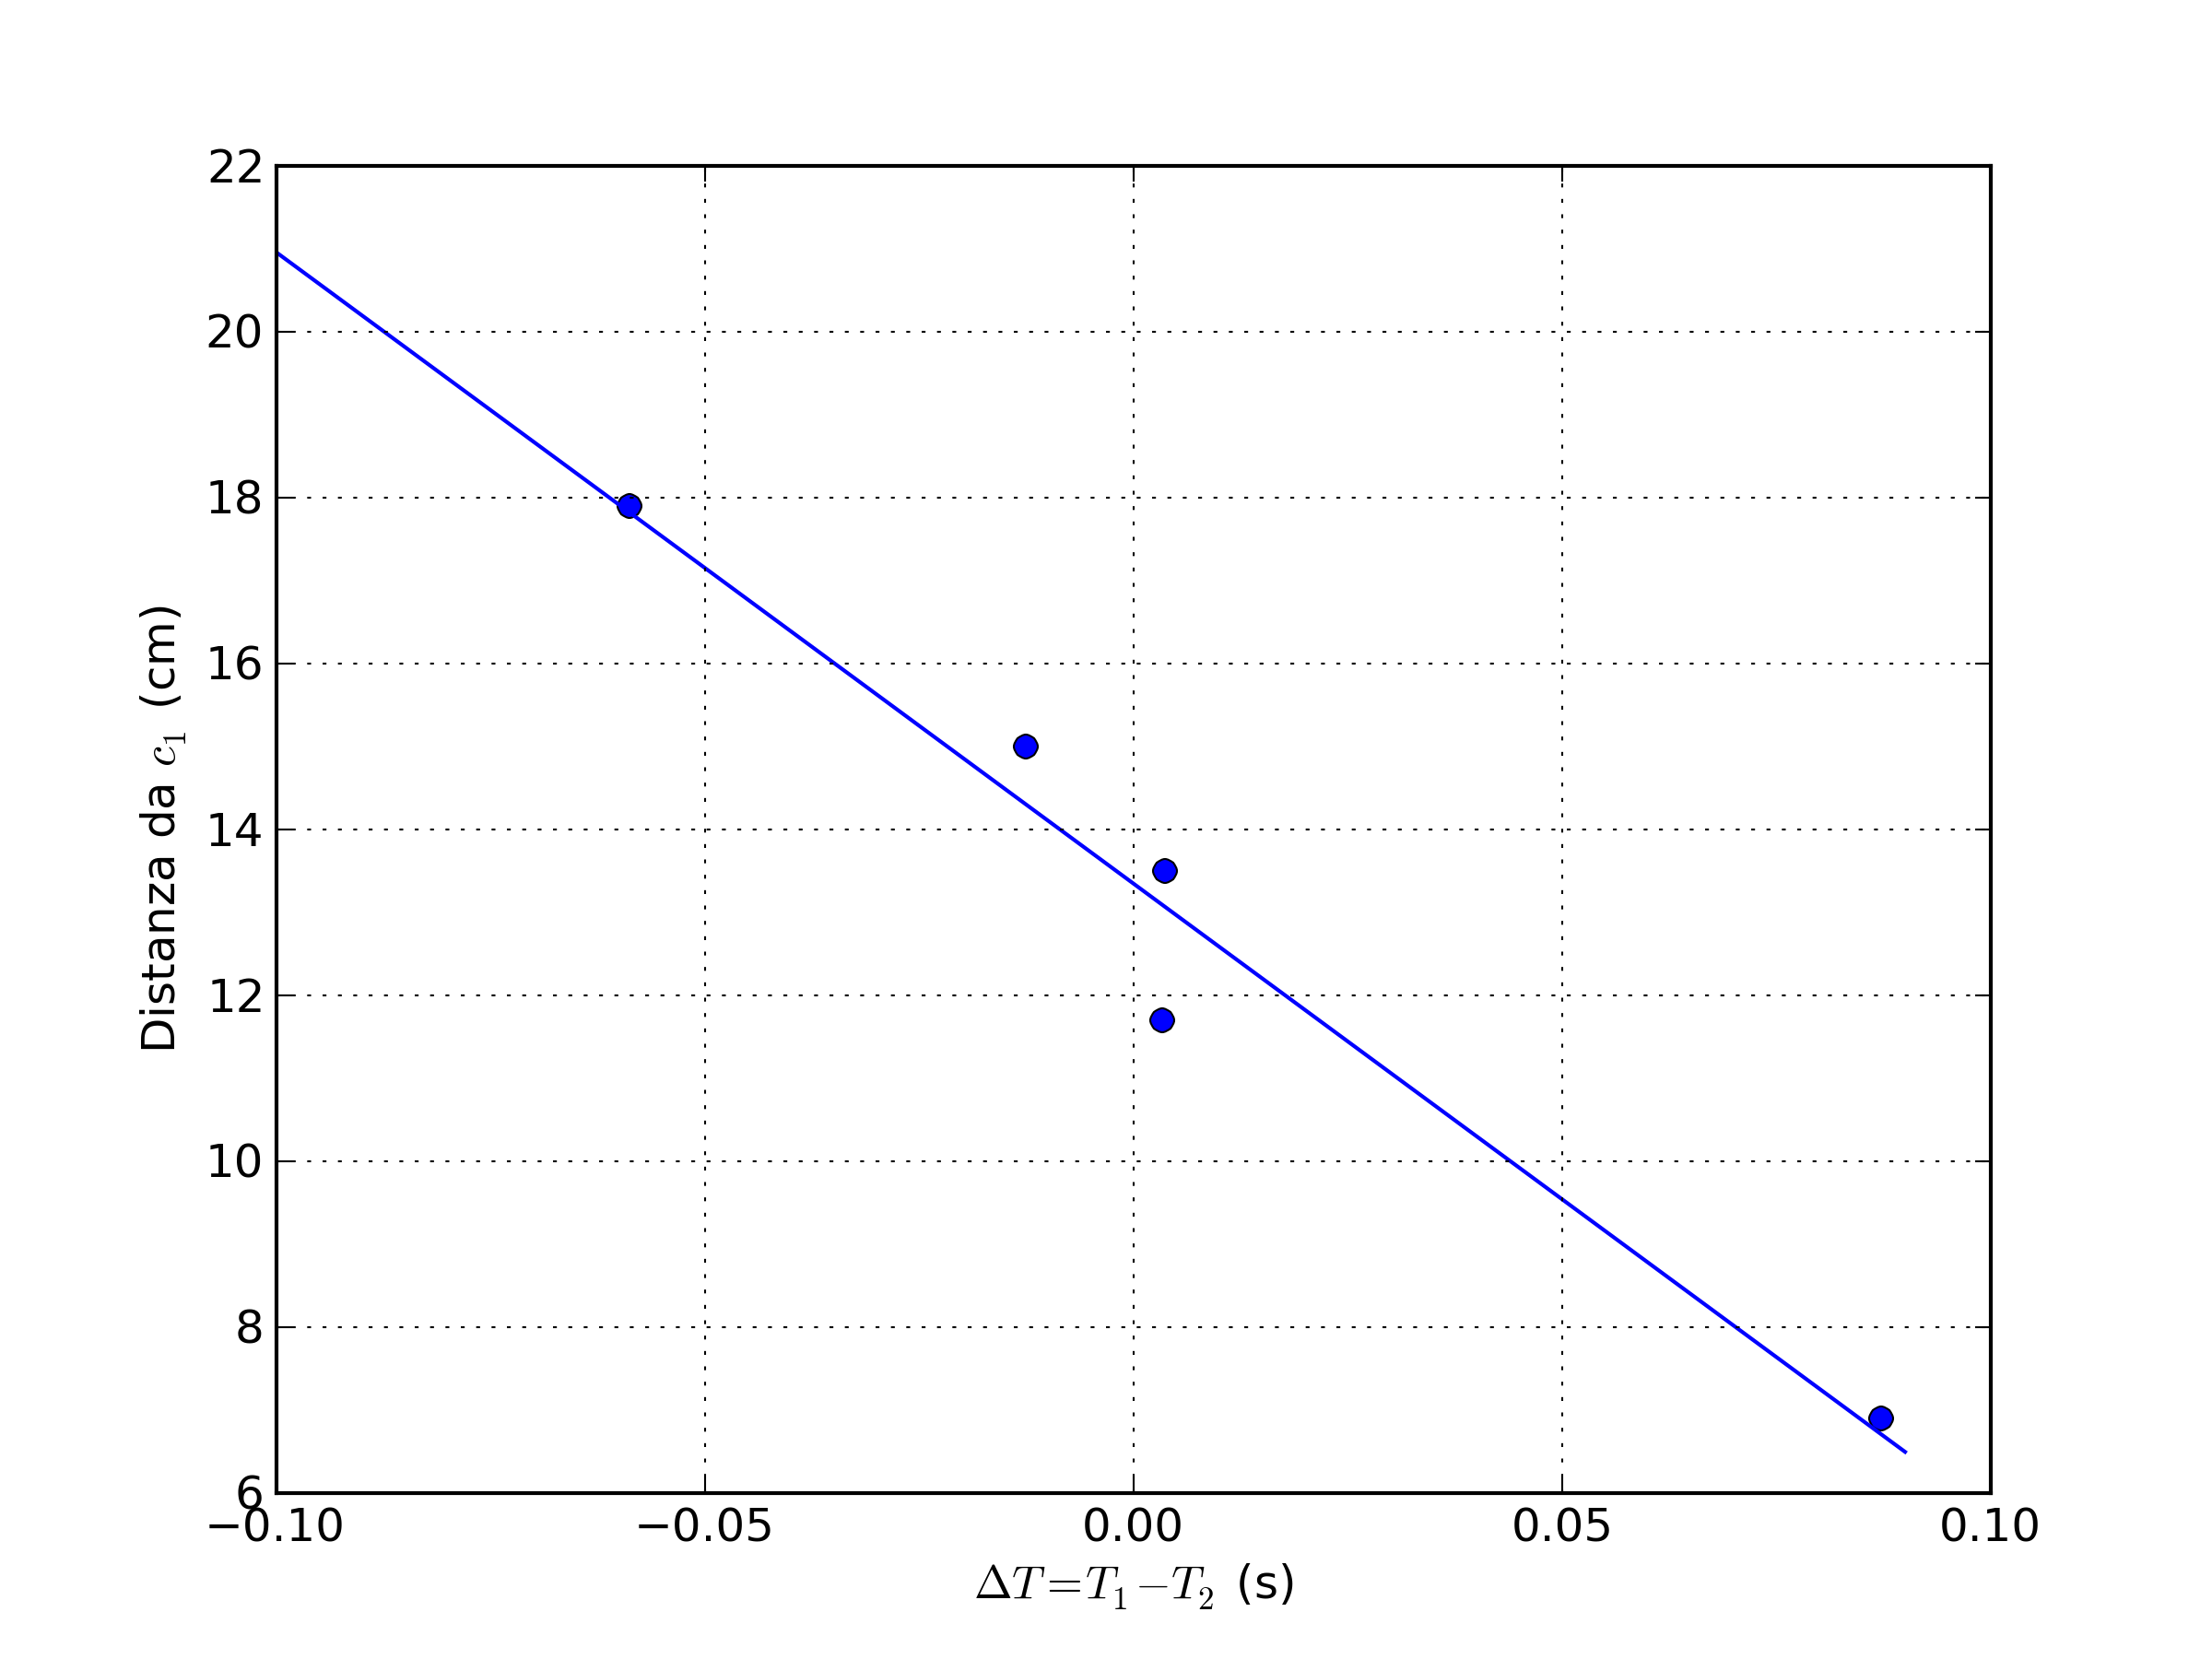
\includegraphics[scale=0.60]{../grafici/kater/intercetta.png}
\end{center}
Il valore così trovato è $d = 13.35 \pm 0.22\ cm$

Trovato il valore $d$, non riuscendo a fare aggiustamenti estremamente precisi alla posizione delle masse, abbiamo preferito calcolare un valore plausibile per il periodo di oscillazione estapolandolo dai valori già trovati. In questo caso abbiamo usato l'interpolazione dei dati di $T_2$ con una retta, in quanto l'interpolazione è migliore rispetto a quella ottenibile interpolando i dati di $T_1$ (e per quanto riguarda $T_2$: $P(\tilde{\chi}^2 \geq \tilde{\chi_0}^2) \geq 11\%$).
In rosso il punto di intersezione trovato, $T^2_0$.

\begin{center}
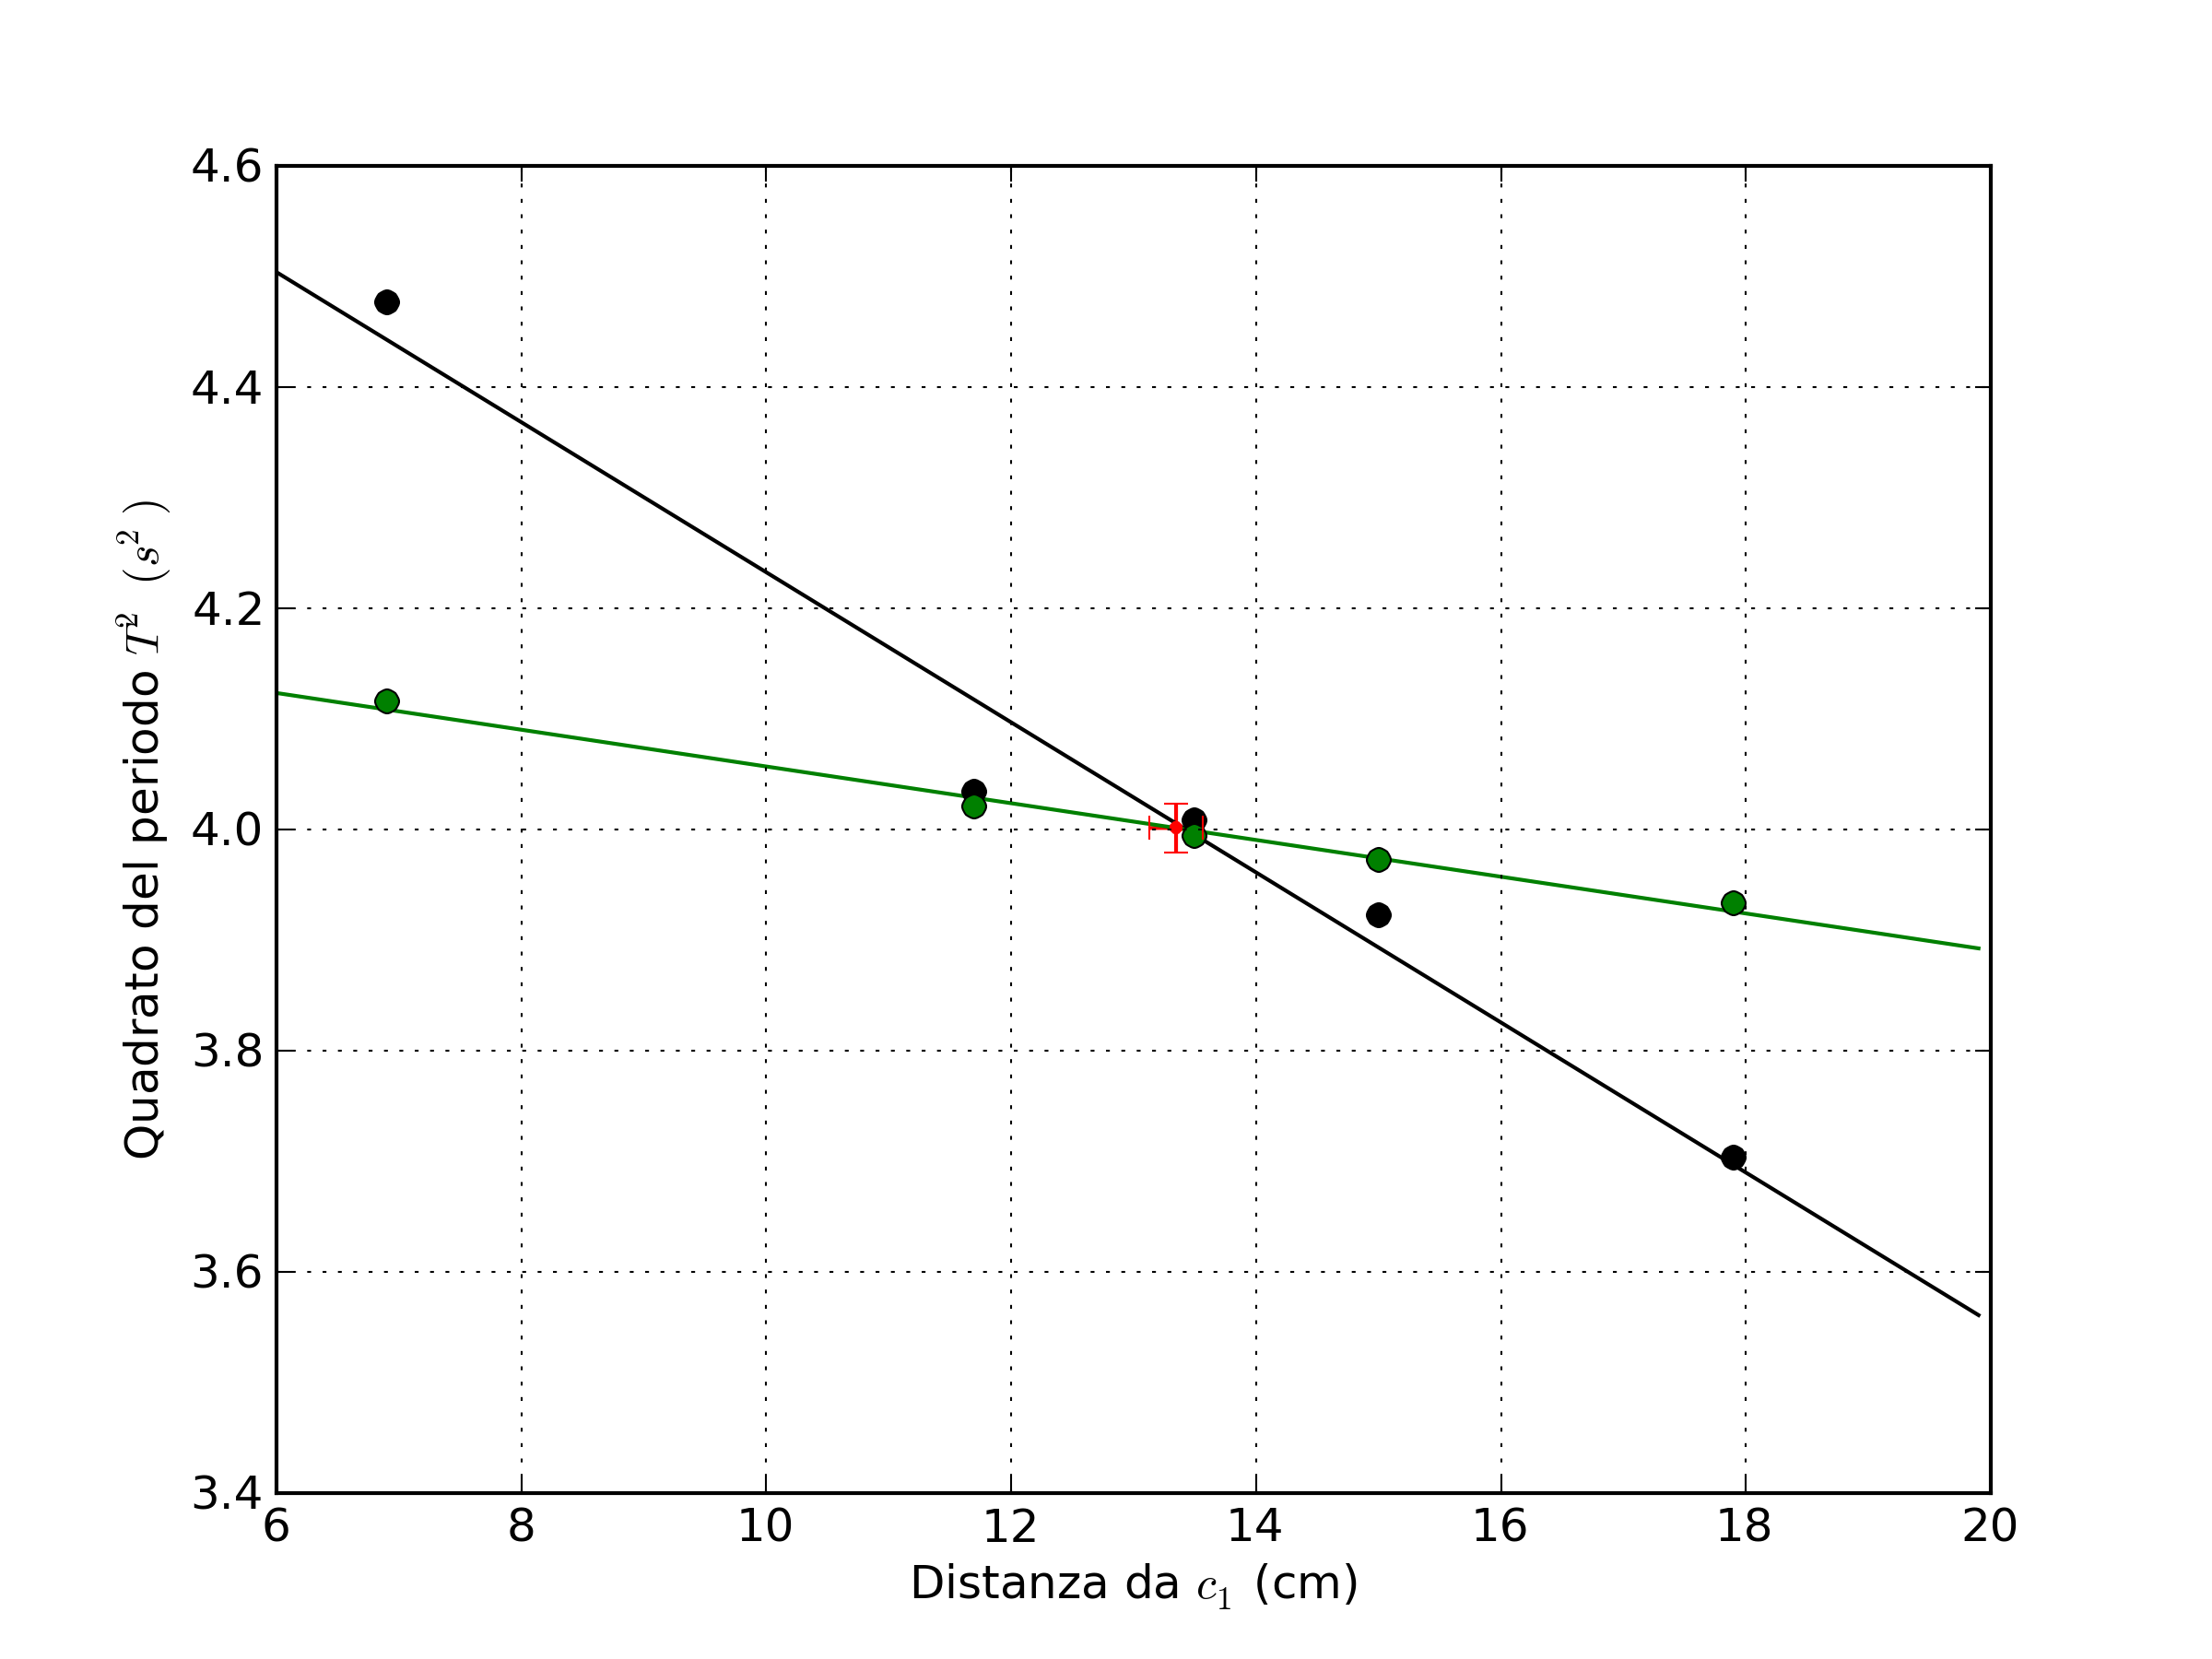
\includegraphics[scale=0.70]{../grafici/kater/intersezione.png}
\end{center}

$$T_0^2 = 4.00\pm 0.03\ s^2$$
Da cui immediatamente si ricava:
$$g = 9.80 \pm 0.07\ m/s^2$$

Vale la pena di spendere qualche parola sul nostro metodo di calcolo delle incertezze qui proposte.

Per calcolare le incertezze su $d$, abbiamo stimato l'errore associato alla misura della distanza della massa mobile dal coltello (in 0.5 cm); abbiamo invece considerato trascurabili le incertezze sulla misura dei tempi, e successivamente abbiamo applicato la normale equazione per il calcolo dell'incertezza in una regressione lineare.
Una volta calcolato questo termine ($\sigma_d = 0.2246\ cm$) abbiamo considerato, utilizzando la stima delle incertezze a posteriori, l'incertezza nell'interpolazione di $T_2$. A questo punto è evidente che, chiamando $\sigma_m$ l'errore sul coefficiente angolare della retta e $\sigma_q$ quello sull'intercetta:
$$T^2_{0\ max} = (m+\sigma_m)(d-\sigma_d) + \sigma_q = 4.03151\ s^2$$
$$T^2_{0\ min} = (m-\sigma_m)(d+\sigma_d) - \sigma_q = 3.97081\ s^2$$
da cui chiaramente si ricava $g_{max}$, $g_{min}$ e dunque:
$$\frac{\Delta (T_0^2)}{2} = \sigma_{T_0^2} = 0.0303\ s^2$$
$$\frac{\Delta g}{2} = \sigma_g = 0.0743\ m/s^2 $$

procedendo poi ad un'ovvia riduzione delle cifre significative a seconda dei dati originali. Abbiamo utilizzato questo metodo per trovare l'intervallo più ampio entro il quale poteva essere compresa la nostra misura, non avendo a nostra disposizione metodi più accurati. Bisogna notare che, nonostante ciò, la misura di $g$ è particolarmente vicina al valore generalmente accettato, specialmente per quanto riguarda il valore medio.

Infatti, considerando $g=9.81\ m/s^2$, ovvero la media dell'accelerazione di gravità sulla superficie terrestre:
$$\frac{\sigma_g}{g} \simeq 0.76\% $$


\section{Caduta libera}
\subsection{Procedimento}
L'apparato sperimentale per misurare l'accelerazione di gravit
\subsection{Raccolta dati}
Tutti i valori riportati in tabella sono in millisecondi.
\begin{center}
\begin{tabular}{r|*{14}{c}}
\textbf{20 cm} & 197 & 199 & 197 & 200 & 199 & 203 & 200 & 203 & 196 & 199 & 196 & 199 & 197 & 205\\
& 198 & 199 & 198 & 197 & 199 & 198 & 197 & 198 & 200 & 198 & 199 & 199 & 198 & 204\\
\midrule
\textbf{35 cm} & 265 & 265 & 265 & 261 & 262 & 263 & 266 & 262 & 269 & 266 & 261 & 263 & 262 & 261\\
\midrule
\textbf{50 cm} & 314 & 315 & 314 & 321 & 319 & 316 & 315 & 315 & 315 & 314 & 314 & 315\\
\midrule
\textbf{60 cm} & 347 & 345 & 346 & 347 & 344 & 344 & 348 & 345 & 346 & 344 & 345 & 345\\
\midrule
\textbf{90 cm} & 424& 424& 424& 423& 425& 424& 426& 423& 424& 423& 422& 425& 423\\
\end{tabular}
\end{center}

\begin{center}
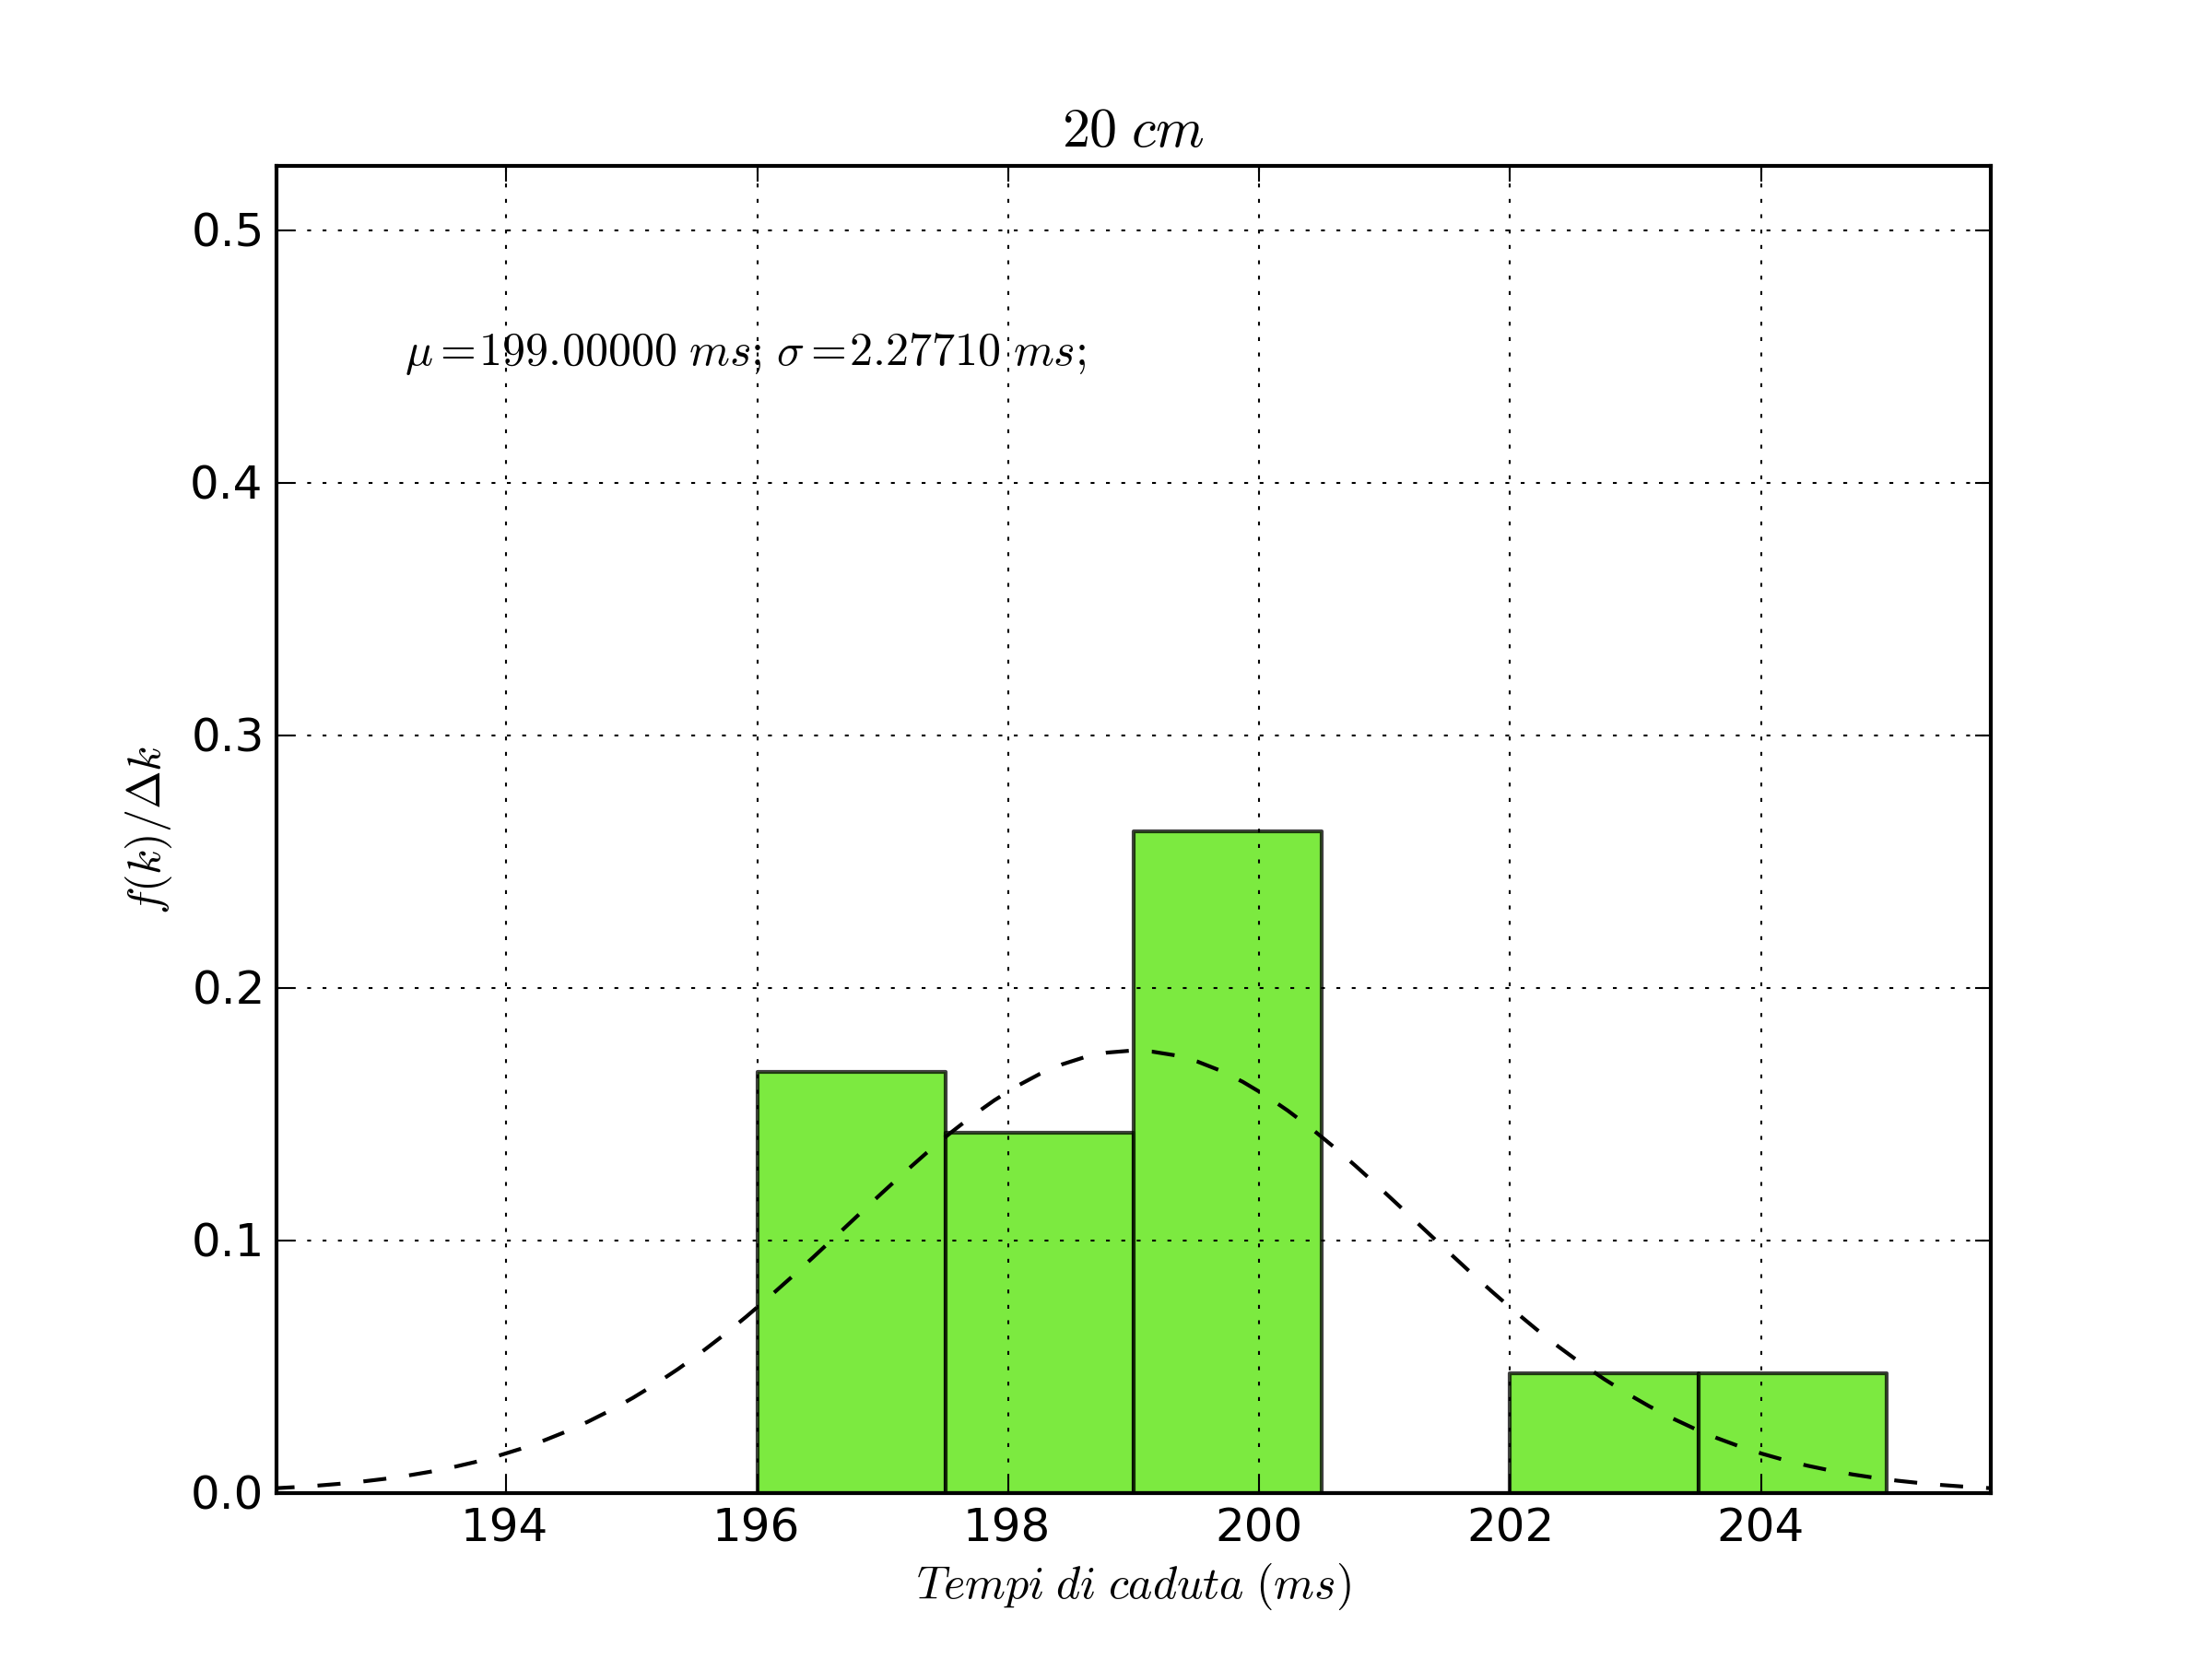
\includegraphics[scale=0.70]{../grafici/20cm.png}
$$\sigma_g = \frac{-4y}{t^3}\sigma_t $$
$$\sigma_{\bar{t}} = 0.430\ ms$$
$$\mathrm{Stima\ di\ g} = 10.10\ m/s^2$$
$$\mathrm{Stima\ (con\ corr.)\ di\ g} = 9.80\ m/s^2 $$
$$\frac{\Delta g_c}{g} = 0.00072$$
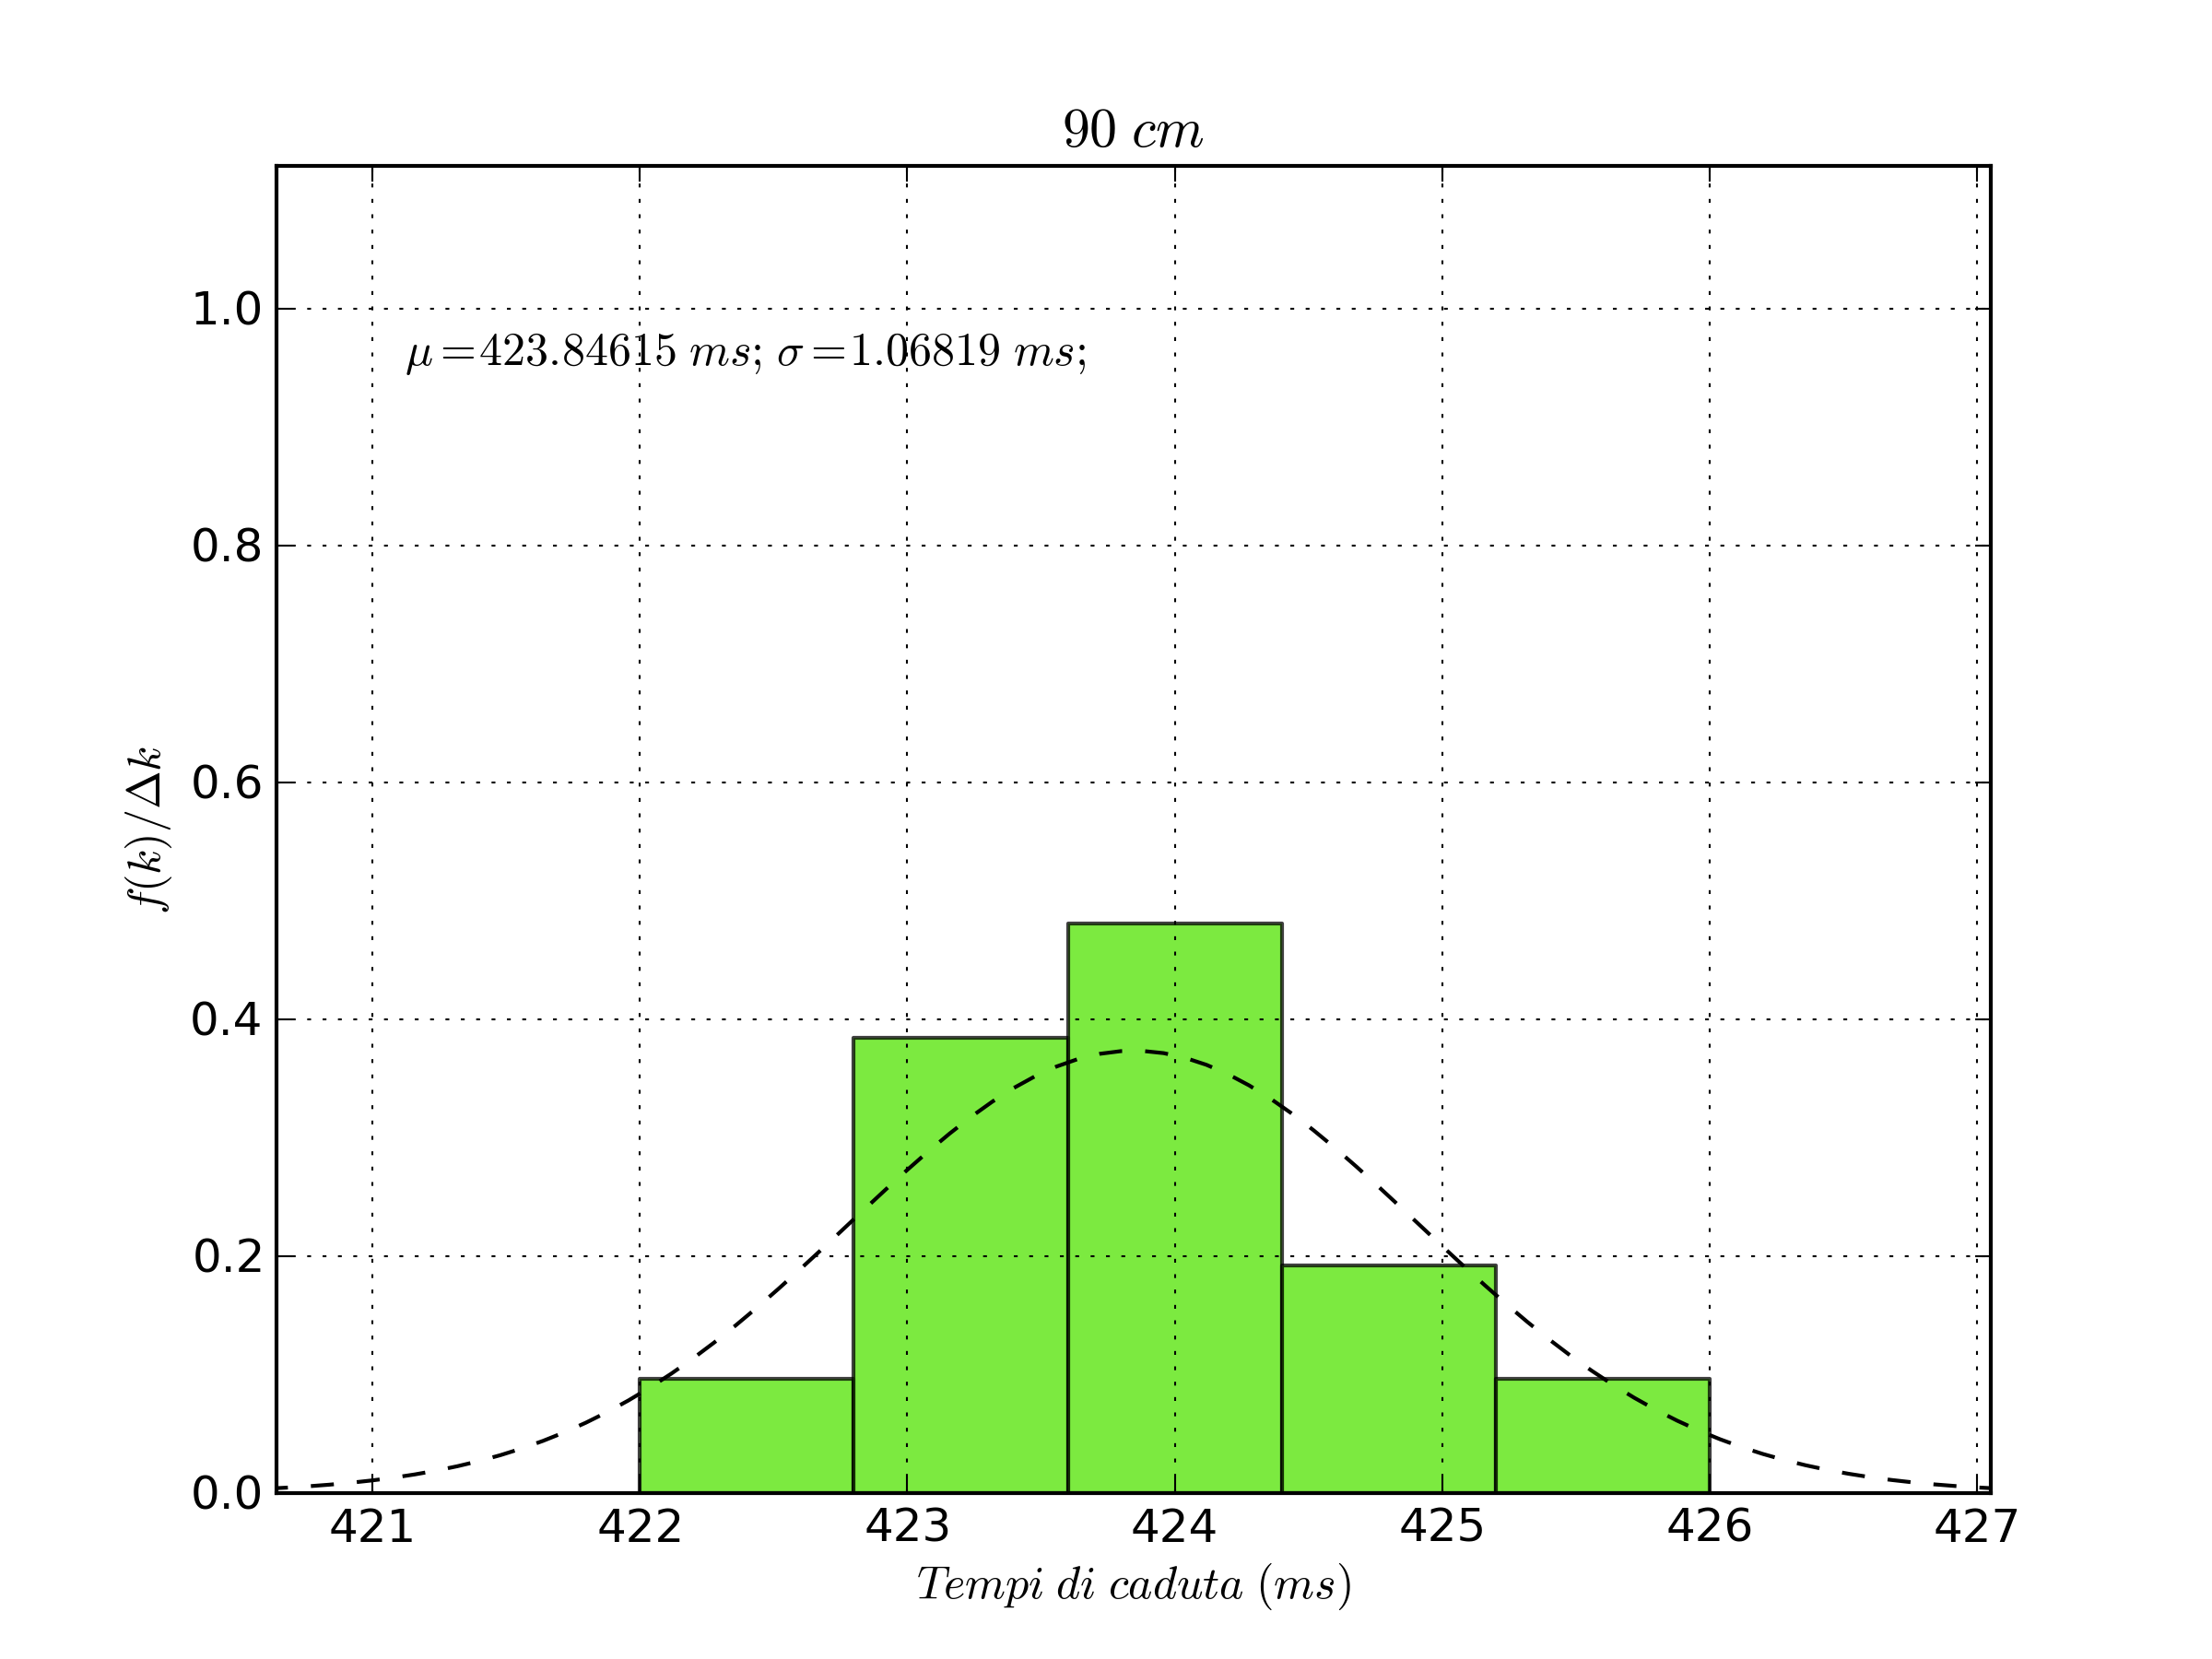
\includegraphics[scale=0.70]{../grafici/90cm.png}
$$\sigma_{\bar{t}} = 0.296\ ms $$
$$\mathrm{Stima\ di\ g} = 10.02\ m/s^2$$
$$\mathrm{Stima\ (con\ corr.)\ di\ g} = 9.88\ m/s^2 $$
$$\frac{\Delta g_c}{g} = 0.00707$$
\end{center}

La correzione applicata è di 3 ms aggiunti al tempo segnato dal cronometro. Non avendo dati più precisi sulla costruzione dell'apparato, assumiamo questo tempo come tempo di risposta dell'intero strumento. In tabella sono riportati i vari valori di $g$, $g_c$ e della distanza di questa misura dal valore vero (in percentuale).

\begin{center}
\begin{tabular}{c|c|c|c|c}
$h$ (m) & $g$ (m/s$^2$) & $g_c$ (m/s$^2$) & $\Delta g/g$ & $\Delta g_c/g$\\
\midrule
0.20 & 10.10 & 9.80 & 0.02964 & 0.00072 \\
0.35 & 10.07 & 9.85 & 0.02659 & 0.00362 \\
0.50 & 10.04 & 9.85 & 0.02354 & 0.00435 \\
0.60 & 10.05 & 9.88 & 0.02475 & 0.00718 \\
0.90 & 10.02 & 9.88 & 0.02138 & 0.00707 \\
\end{tabular}
\end{center}


\section{Conclusioni}
Nonostante 

